\documentclass[11pt]{article}
\setlength{\oddsidemargin}{0in}
\setlength{\evensidemargin}{0in}
\setlength{\textwidth}{6.5in}
\setlength{\parindent}{0in}
\setlength{\parskip}{\baselineskip}

\usepackage{url}

\usepackage{amsmath}
\usepackage{amsthm}
\usepackage{amssymb}
\usepackage[dvips]{graphics}
\usepackage{epsfig}
\usepackage{color}
\usepackage{fullpage}
\newcommand{\F}{{\mathbb F}}

\begin{document}
\begin{center}
{\Large \bf Math 175: Combinatorics} \\
{\Large \bf Homework 5}\\
{\Large Posted Friday February 16\\
Due in Discussion Section Thursday February 22}
\end{center}

\vspace{5mm}

After the last homework we started by discussing some examples about counting labeled versus unlabeled teams.  We explained why there is less than a 50\% chance that you end up on the same team as your friend.

We then introduced the subtraction principle.  The main idea is that we want to count sequences/outcomes with some property.  We instead count the total number of possible sequences/outcomes and then subtract off the number of sequences/outcomes without this property.  We gave examples involving people sitting around a circular table.  There is no section of our textbooks that goes over the subtraction principle specifically, but these ideas can be applied to several of the problems in Chapter 1 of LVP.

We discussed lattice paths on a grid and the Catalan numbers.  We showed that there are $\binom{n+m}{m}$ paths of length $n+m$ from $(0,0)$ to $(m,n)$.  When $n=m$ we showed that the number of these paths that do not cross above the diagonal line $x=y$ is given by the Catalan number $C_n$.  We did this by using the reflection principle to show that the number of paths that do cross above $x=y$ is given by $\binom{2n}{n-1}$.  

We spent a lecture highlighting the diversity of things that are counted by Catalan numbers. 

Catalan numbers are the subject of Section 2.6.6 of the HHM book, but the perspective is very different.  The Wikipedia entry for Catalan numbers does a good job presenting the material that we covered on this topic.  

We then gave some examples involving the Pigeonhole principle.  This is the subject of Section 2.4 in LVP and Section 2.4 in HHM.  

%Finally, we started to talk about the Principle of Inclusion-Exclusion.  This is the subject of Section 2.3 of LVP and Section 2.5 of HHM.

%If you would like to get a head start on reading for next week, I recommend going over the proof of Theorem 2.6 on page 158 of HHM and the section on Derangements starting on page 160.

\newpage

\center{\Large Problems}

\begin{enumerate}

\item 
\begin{enumerate}
\item How many ways are there to line up $4$ boys and $8$ girls so that no two boys are next to each other?  

{\bf Note}: Each child is a unique, so $B_1 B_2 B_3 B_4 G_1 G_2 \cdots G_8$ is a different lineup than $B_2 B_1 B_3 B_4 G_1 G_2 \cdots G_8$, (although neither one counts for this question.)

\item How many ways are there to seat these $4$ boys and $8$ girls at a circular table (with $12$ labeled chairs) so that no two boys are next to each other?
\end{enumerate}

\item How many pairs of subsets $A, B$ of $\{1,2,\ldots, n\}$ are there such that $A$ is contained in $B$?

\item Let $C_n = \frac{1}{n+1} \binom{2n}{n}$.  Show that for $n\ge 1$
\[
C_n = \sum_{k=0}^{n-1} C_k C_{n-1-k}.
\]
{\bf Hint}: Can you think of a way to break up a path from $(0,0)$ to $(n,n)$ that does not cross above the diagonal line $x=y$ into two parts?

\item Nathan and Amir are running for President of Math 175.  There are $2n+1$ students voting in the election.  Each student writes their favorite candidate's name on a piece of paper and throws it in a box.  The ballots are shuffled and then counted one by one.  This particular election is extremely close- Nathan wins by a single vote.

What is the probability that once the first ballot is read out, Nathan is strictly ahead of Amir for the entire ballot counting process?

{\bf Example}: When there are $5$ votes, N gets $3$ and A gets $2$.  Here is one possible way for the ballots to be read out where Nathan is always ahead: NNANA.  The reading NNAAN does not count, because after four votes are read the candidates are tied.

\item Suppose $2k$ people are seated around a table with labeled chairs.  How many ways are there for $k$ pairs of people to shake hands simultaneously across the table in such a way that no arms cross?

\begin{figure}[h]
\centering
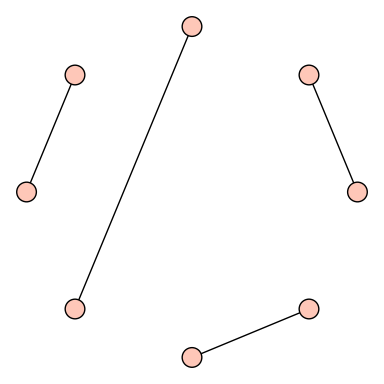
\includegraphics[width=30mm]{oct.png}
\caption{A way for $n = 8$ people to shake hands with no arms crossing}
\end{figure}

{\bf Hint}: By setting up Segners recursion, show that the number of ways for $n$ pairs of people to do this is the $n$th Catalan number. 

%\item A diagonal of a convex polygon is a line segment connecting two non-adjacent vertices of the polygon.  Let $p_n$ denote the number of ways to decompose a convex polygon having $n$ vertices into triangles by drawing $n-3$ diagonals that do not cross inside the polygon.  Assume the vertices of the polygon are labeled, so that triangulations with different orientations are counted separately.


%\begin{figure}[h]
%\centering
%\includegraphics[width=30mm]{hex.png}\ \ \ \ \ \includegraphics[width=30mm]{hex1.png}
%\caption{Two distinct triangulations for $n = 6$}
%\end{figure}


%\begin{enumerate}
%\item Determine $p_3, p_4$ and $p_5$ by showing all possible triangulations.
%\item Let $v$ be a fixed vertex of a polygon with $n=6$ sides.  Count all the triangulations of the hexagon by considering two cases: (i) $v$ is not an endpoint of any of the three diagonals added in the triangulation, and (ii) $v$ is an endpoint of at least one of the diagonals.  Use this to determine the value of $p_6$ without drawing every possible triangulation.
%\item Find a formula for $p_n$ and prove that it holds for all $n$.
%\end{enumerate}

%\vspace{1 cm}

\item In class we saw that the number of paths from $(0,0)$ to $(m,n)$ of the minimal length $m+n$ is $\binom{m+n}{m}$.  We saw that the number of these paths passing through $(a,b)$ is given by
\[
f_{m,n}(a,b) = \binom{a+b}{a} \cdot \binom{(m+n)-(a+b)}{m-a}.
\]
For any $n \ge 1$, it is clear from the definition that $f_{n,n}(1,1) = f_{n,n}(n-1,n-1)$. Show that for any $a$ satisfying $1< a < n-1$,
\[
f_{n,n}(1,1)  > f_{n,n}(a,a).
\]
{\bf Hint}: What can you say about the ratio $f_{n,n}(a,a)/f_{n,n}(a+1,a+1)$?

\item Suppose there are $m+n$ students in a class, $a+b$ of them are girls, and $m \ge a$.  If we randomly choose $m$ students, what is the probability that exactly $a$ of them are girls?

\item We select $38$ even positive integers all less than $1000$.  Prove that there will be two of them whose difference is at most $26$.

\item \begin{enumerate}
\item Show that any $4$-element subset of $\{1,2,\ldots, 6\}$ has two disjoint subsets that have the same sum. 

{\bf Hint}: Argue by contradiction. 

\item Show that there is a $4$-element subset of $\{1,2,\ldots, 7\}$ such that no two disjoint subsets have the same sum.
\end{enumerate}

\item Suppose we shoot five arrows at a target that is $6$ inches by $6$ inches.  Since we are awesome at archery (no big deal) we hit the target every time.  Prove that there are two arrows with distance between them at most $3\sqrt{2}$ inches.



\end{enumerate}


\end{document}